\chapter{Preliminary Evaluation}
\label{chapter:preliminary_evaluation}
To answer the research questions (see \autoref{chapter:introduction} for more information), we conducted a preliminary evaluation. In the small scope of this evaluation, we wanted to learn about the status and moods knowledge workers share with their closest team members, what they learn from their interactions with their teammates and the overall impact on their perceptions of isolation in the workplace. The feedback can then be used to develop both the study and the tool further.

The timeline of the preliminary evaluation is shown in \autoref{fig:study_timeline}. Before the study was officially launched with the kick-off meeting with the entire team, each participant was asked to sign and return the consent form (see \autoref{chapter:consent_form}). In addition, each participant was asked to complete a questionnaire that included some demographic questions and a 10-item questionnaire about their perception of isolation in the workplace. During the kick-off meeting, participants were given the opportunity to ask any questions about the consent form. The goal of the kick-off meeting was to install AmbientTeams and show the team each of the features. Following the kick-off meeting, AmbientTeams was deployed for at least three working days (in our case, it was five). After that, but before the final meeting, another questionnaire was sent to the participants to have a before and after comparison. Last but not least, a final interview was conducted with each participant individually to get more qualitative insights.

\begin{figure}[h]
    \centering
    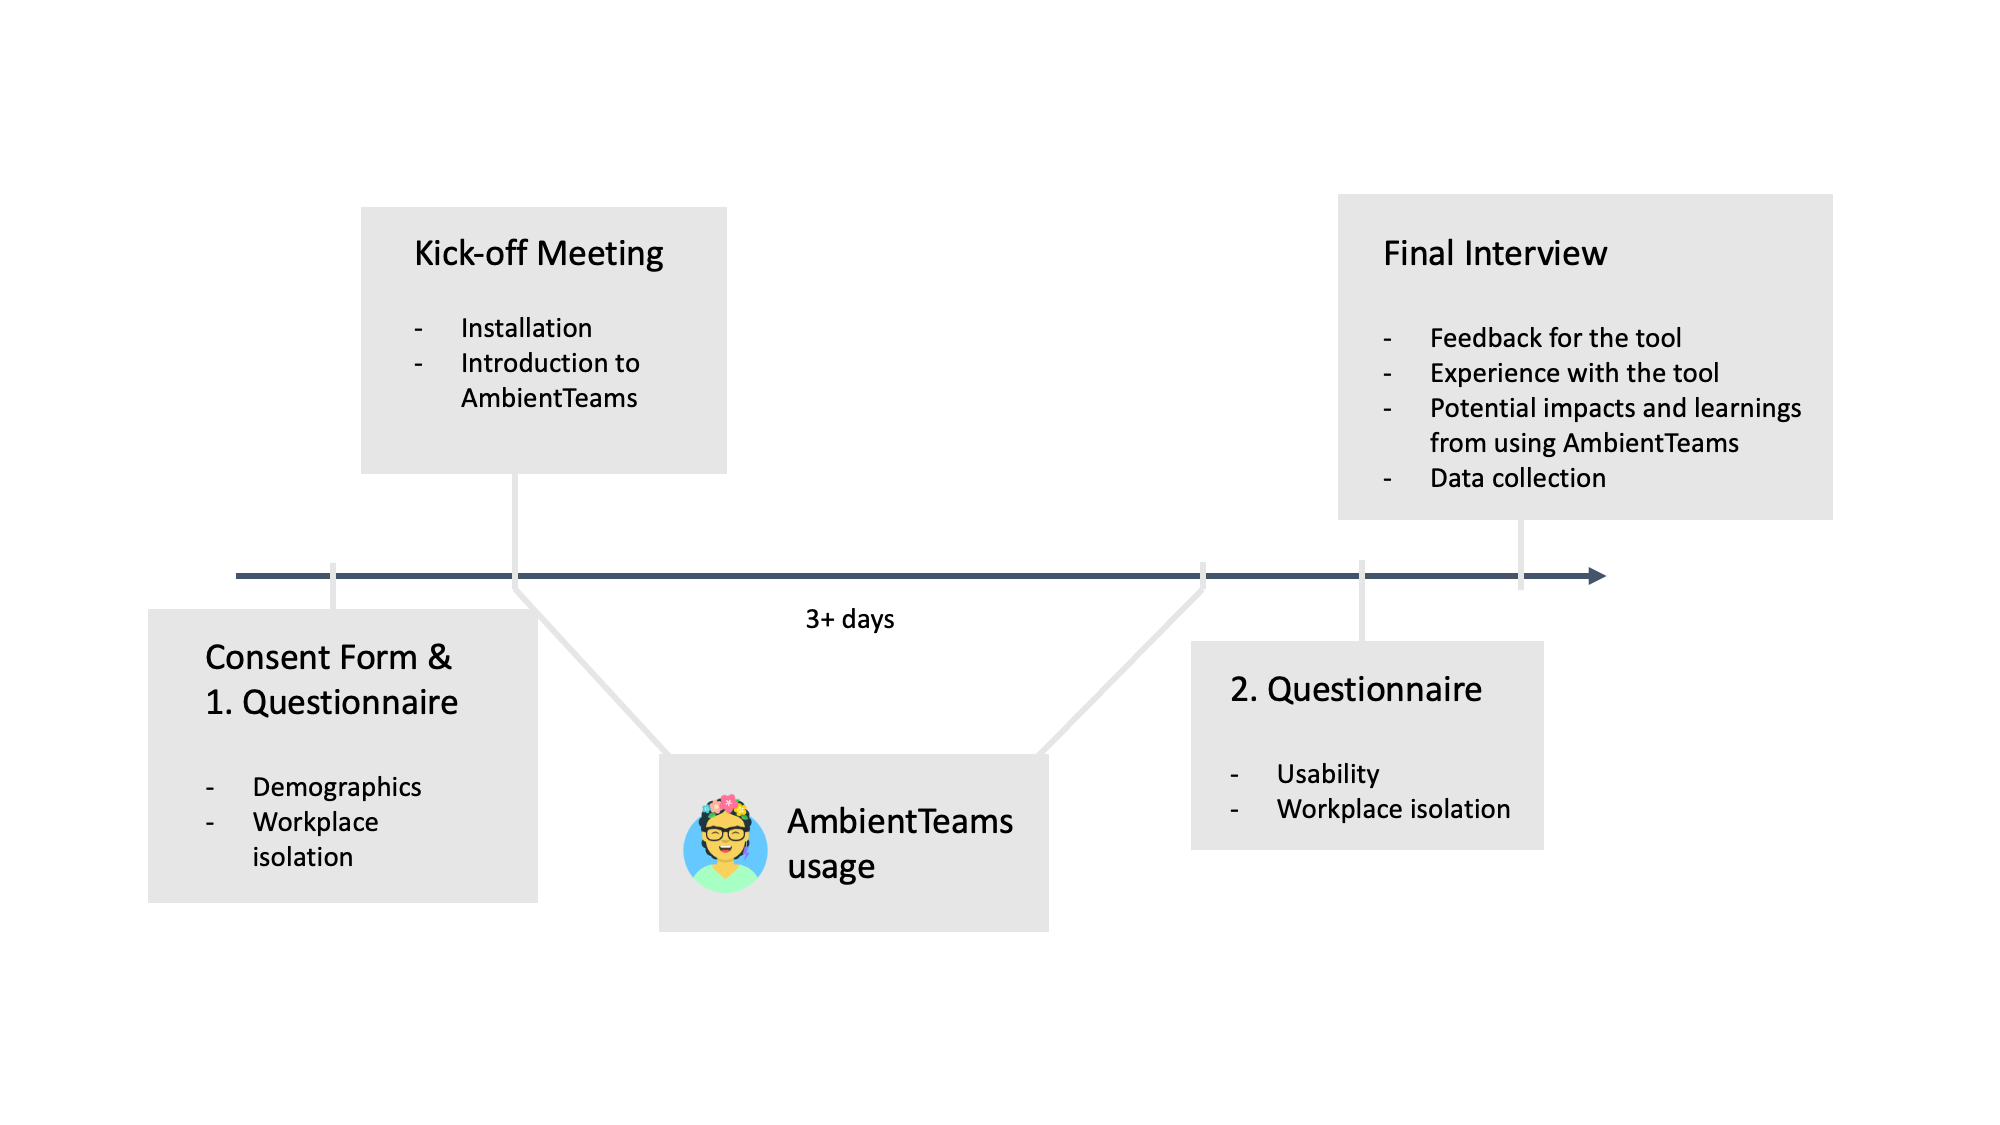
\includegraphics[width=.8\linewidth]{./images/Study_Timeline.png}
    \caption{Study Timeline}
    \label{fig:study_timeline}
\end{figure}

In the following sections, we present more details about the study procedure.

\section{Participants Recruitment}
\label{section:recruitment}
The first step was to recruit an interested team. The researchers' network was used for this purpose. For this purpose, the study description was forwarded to personal contacts. Once an interested team was identified, it was checked whether it met the participation criteria and whether the potential participants were allowed to install AmbientTeams on their computer (technically speaking). If this was not the case, the company's consent and permission to install AmbientTeams were first obtained. To inform the company as much as possible about the study and the confidentiality of the data collected, the consent form and a study description were given to the company for review. After obtaining the company's consent, interested team members were approached individually by introducing the study, discussing the steps and objectives of the study, and emphasizing that participation is completely voluntary. In order for participants to remain anonymous, each participant was assigned a random pseudonym, e.g., P392, which had to be given as the response to the first question in both questionnaires. The requirements for participating teams were:

\begin{enumerate}
    \item At least three team members
    \item Three or more common working days a week
    \item Spending the majority of their workday on the computer
    \item Working remotely as much as possible (ideally completely remote)
    \item Having all the required rights to install AmbientTeams on their work computer
    \item Willingness to use AmbientTeams during at least three full days of work
    \item Using macOS or Microsoft Windows
    \item An active internet connection
\end{enumerate}

\section{Pre-Study Questionnaire}
\label{section:prestudy_questionnaire}
The pre-study questionnaire includes some basic demographic questions as well as an established workplace isolation questionnaire developed by \textcite{marshall2007workplace}. The demographic questions ask about age, gender, work industry, work experience, and job title. Questions are also asked about the current culture of communication within the team, whether they are aware of their colleagues' feelings and progress, and preferred work style (remote vs. onsite). The Workplace Isolation Questionnaire was used as a baseline measure. The same questionnaire was also asked at the end of the study, prior to the final interview, to gain possible initial insights into whether our approach could reduce perceptions of workplace isolation among knowledge workers. The workplace isolation questionnaire contains ten questions and uses a 7-point Likert scale, with 1 representing \enquote{strongly disagree} and 7 representing \enquote{strongly agree}. Finally, participants could optionally write down their expectations for the study. The complete pre-study questionnaire can be found in \autoref{chapter:prestudy_questionnaire}.

\section{Initial Meeting}
\label{section:initial_meeting}
Due to the relatively small number of team members and their flexibility, it was possible to hold a kick-off meeting with the entire team. During this meeting, the consent form (see \autoref{chapter:consent_form}) and study instructions (see \autoref{chapter:study_instructions}) were briefly reviewed, and there was an opportunity to ask questions. We then walked participants through the installation process and explained and demonstrated the functionality of AmbientTeams. Finally, each participant joined the team we had created prior to the meeting. After the kick-off meeting, the study period officially began.

\section{Evaluation Phase}
\label{section:evaluation}
The team was happy to use AmbientTeams for a workweek (five days) instead of the originally planned three days. During this time, participants were instructed to continue working as usual. Further, participants were instructed to contact us if there was a problem or if they had any other feedback. For very brief feedback, AmbientTeams also has a simple feedback sending feature. During this evaluation phase, usage data of the application were collected from each participant. For this purpose, \autoref{table:data} shows an overview of all collected data and for which research question it is relevant, along with the location of storage (local or server). Local refers to the participants' computers, while server refers to the server hosted at the Institute of Computer Science at the University of Zurich. In other words, the data stored on the server is automatically shared with the researchers, whereas only the participants can access the locally stored data unless they explicitly share this data with us at the end of the study.

\begin{table}[h] \footnotesize
    \centering
    \begin{tabularx}{.9\textwidth}{l X l l}
        \toprule
        Entity                               & Data collected                         & Storage                 & RQ Relevance                  \\
        \midrule
        \multirow{5}{*}{User}                & email                                  & \multirow{5}{*}{Server} & \multirow{5}{*}{-}            \\
                                             & display name                           &                         &                               \\
                                             & hashed password                        &                         &                               \\
                                             & the teams the user belongs to          &                         &                               \\
                                             & avatar created on signup               &                         &                               \\
        \midrule
        \multirow{2}{*}{Team}                & name of the team                       & \multirow{2}{*}{Server} & \multirow{2}{*}{-}            \\
                                             & belonging team members                 &                         &                               \\
        \midrule
        \multirow{4}{*}{Status message}      & timestamp                              & \multirow{4}{*}{Server} & \multirow{4}{*}{RQ2, RQ4    } \\
                                             & text content of the status             &                         &                               \\
                                             & team where status was posted           &                         &                               \\
                                             & user the status belongs to             &                         &                               \\
        \midrule
        \multirow{4}{*}{Direct message}      & timestamp                              & \multirow{4}{*}{Server} & \multirow{4}{*}{RQ2, RQ4    } \\
                                             & content of the message                 &                         &                               \\
                                             & team where message was sent            &                         &                               \\
                                             & user the message belongs to            &                         &                               \\
        \midrule
        \multirow{3}{*}{Availability status} & timestamp                              & \multirow{3}{*}{Server} & \multirow{3}{*}{RQ4}          \\
                                             & selected availability status           &                         &                               \\
                                             & user who posted                        &                         &                               \\
        \midrule
        \multirow{3}{*}{Direct call}         & start/end timestamp                    & \multirow{3}{*}{Server} & \multirow{3}{*}{RQ4}          \\
                                             & participants                           &                         &                               \\
                                             & success: true or false                 &                         &                               \\
        \midrule
        \multirow{3}{*}{Breakroom}           & team                                   & \multirow{3}{*}{Server} & \multirow{3}{*}{RQ4}          \\
                                             & teamMembers                            &                         &                               \\
                                             & start/end timestamp                    &                         &                               \\
        \midrule
        \multirow{4}{*}{Nudge}               & sending/receiving user                 & \multirow{4}{*}{Server} & \multirow{4}{*}{RQ4}          \\
                                             & teamId                                 &                         &                               \\
                                             & start/end timestamp                    &                         &                               \\
                                             & ending user and type                   &                         &                               \\
        \midrule
        \multirow{4}{*}{Random call}         & involved users                         & \multirow{4}{*}{Server} & \multirow{4}{*}{RQ4}          \\
                                             & teamId                                 &                         &                               \\
                                             & start/end timestamp                    &                         &                               \\
                                             & succes: true or false                  &                         &                               \\
        \midrule
        \multirow{3}{*}{Mood}                & timestamp                              & \multirow{3}{*}{Server} & \multirow{3}{*}{RQ2, RQ4}     \\
                                             & selected mood                          &                         &                               \\
                                             & user who shared                        &                         &                               \\
        \midrule
        \multirow{2}{*}{Feedback}            & text content content                   & \multirow{2}{*}{Server} & \multirow{2}{*}{-}            \\
                                             & user                                   &                         &                               \\
        \midrule
        \multirow{4}{*}{Window action}       & opening timestamp                      & \multirow{4}{*}{Local}  & \multirow{4}{*}{RQ4    }      \\
                                             & minimizing timstamp                    &                         &                               \\
                                             & closing timestamp                      &                         &                               \\
                                             & restoring timstamp                     &                         &                               \\

        \midrule
        \multirow{2}{*}{Application action}  & starting timestamp                     & \multirow{2}{*}{Local}  & \multirow{2}{*}{RQ4    }      \\
                                             & quitting timestamp                     &                         &                               \\

        % \midrule
        % \multirow{2}{*}{Team changes}        & timestamp                              & \multirow{2}{*}{Local}  & \multirow{2}{*}{RQ4    }      \\
        % & destination team                       &                         &                               \\

        \midrule
        \multirow{6}{*}{Active windows}      & title: e.g. 'Unicorns - Google Search' & \multirow{6}{*}{Local}  & \multirow{6}{*}{RQ3, RQ4}     \\
                                             & id: e.g. '5762'                        &                         &                               \\
                                             & bounds: x, y, height, width            &                         &                               \\
                                             & owner: owning process                  &                         &                               \\
                                             & url: if application is a web browser   &                         &                               \\
                                             & memoryUsage: e.g. '11015432'           &                         &                               \\
        \bottomrule
    \end{tabularx}
    \caption{Data Collected During the Preliminary Evaluation and Its Relevance for the RQs}
    \label{table:data}
\end{table}

\section{Post-Study Questionnaire}
\label{section:poststudy_questionnaire}
After the evaluation phase, participants were asked to fill out another questionnaire, which takes about 5 minutes, similar to the pre-study questionnaire. In addition to some control questions about the extent to which participants worked remotely during the study and approximately how long AmbientTeams ran in the foreground, a usability questionnaire was presented. Usability is measured based on the results of this questionnaire using the System Usability Score (SUS) introduced by \textcite{brooke1996sus}. As mentioned earlier, the last block of the post-study questionnaire includes the same workplace isolation questionnaire that was already answered in the Pre-Study questionnaire. The full post-study questionnaire can be found in \autoref{chapter:poststudy_questionnaire}.

Together with the pre-study questionnaire, the post-study questionnaire aims to find insights into the potential impact of AmbientTeams on perceived workplace isolation. In addition, the SUS will help us better understand and quantify the usability of our approach.

\section{Semi-Structured Final Interview}
\label{section:interview}
To complement the quantitative data, a semi-structured final interview was conducted with each participant individually. The goal of this interview was to gain valuable insight into the use of AmbientTeams, its strengths, weaknesses, and impacts, as well as the participants' sharing behaviors. All interview questions and their relevance to the research questions can be found in \autoref{chapter:interview_guide}. Interviews were designed to last approximately 45 minutes per participant, including the time needed to export local data at the beginning of the last interview. Due to the potentially confidential information contained in the data collected, participants were free to obfuscate the contents of the active Windows file before uploading it to UZH dropfiles\footnote{\url{https://dropfiles.uzh.ch/}}. We recorded the interviews if the participant allowed and then transcribed them. Two researchers (one of whom is the author of this paper) independently open-coded the transcripts to analyze the interviews.

\section{Participants}
Through our private network of contacts, we were able to find an interested team for the pre-evaluation. The group initially consisted of six knowledge workers working for a Swiss company in the FinTech industry. Unfortunately, one person was eliminated from the study because this person was inactive in using AmbientTeams and could not be reached even after several attempts. The remaining five individuals were three employees who had been with the company for approximately two years. Two had only been with the team for about three months at the time the study began. All participants were between 25 and 34 years old, and their work experience ranged from 3 (working student) to 13 years (senior accountant). Of the five participants, three were female, and two were male.